\section{Results}

The model performed better than using the average
recipe in predicting the U.S. \gls{UNF}. However,
the model underperformed in predicting uranium-235
and uranium-238.


\subsection{Depletion Calculation Time and File Size}

For 100 sets of
burnup and enrichment depletion calculations,
the model takes 0.12 seconds, while
searching the database for an assembly
with the closest burnup and enrichment (using Pandas read csv)
takes 21.8 seconds. Also, the pickled model file is only
38 Kb, while the curated database (.csv) is 330 Mb.

\subsection{Assembly Comparison}

Ten burnup and enrichment data was picked at random from the \gls{UDB},
and was compared with the model predictions, to observe
two things:
\begin{enumerate}
    \item What isotope (or Z, A range) the model is good / bad 
        at predicting
    \item What burnup / enrichment range the model is good / bad
        at predicting
\end{enumerate}

Figures \ref{fig:211_28539}, \ref{fig:33_38632},
\ref{fig:40_29933}, \ref{fig:432_52029} show that the model
generally has a high relative error percentage for Ra-226
(average concentration 6.0 e-12\%) ,Ac-227 (average concentration  2.3 e-12\%), and curium isotopes. It should
be noted that the absolute prediction error is quite small
(\textasciitilde 1e-11), but the percent error is large due
to the small value of the data.

\begin{figure}
    \centering
    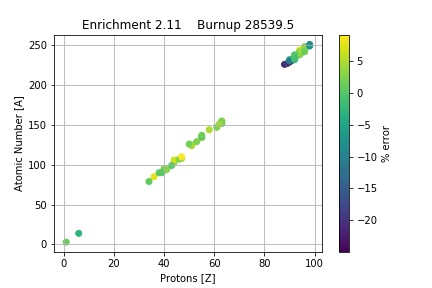
\includegraphics[width=\textwidth]{2-11_28539-5.png}
    \caption{Isotope by isotope prediction error percentage
             plotted for a discrete burnup and enrichment.
             }
    \label{fig:211_28539}
\end{figure}



\begin{figure}
    \centering
    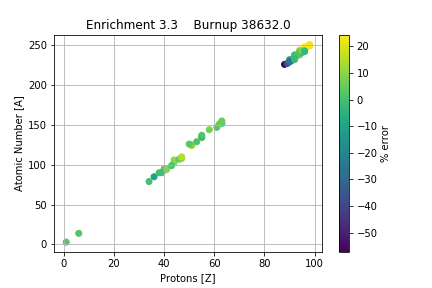
\includegraphics[width=\textwidth]{3-3_38632-0.png}
    \caption{Isotope by isotope prediction error percentage
             plotted for a discrete burnup and enrichment.
             }
    \label{fig:33_38632}
\end{figure}


\begin{figure}
    \centering
    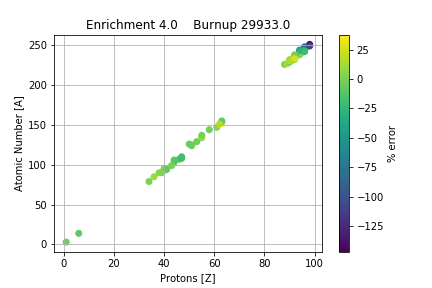
\includegraphics[width=\textwidth]{4-0_29933-0.png}
    \caption{Isotope by isotope prediction error percentage
             plotted for a discrete burnup and enrichment.
             }
    \label{fig:40_29933}
\end{figure}
    

\begin{figure}
    \centering
    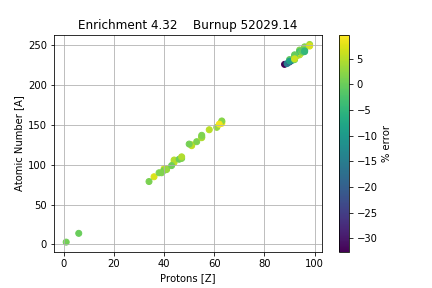
\includegraphics[width=\textwidth]{4-32_52029-14.png}
    \caption{Isotope by isotope prediction error percentage
             plotted for a discrete burnup and enrichment.}
    \label{fig:432_52029}
\end{figure}

\subsection{U.S. \gls{UNF} Inventory Comparison}

In this section we compare three values:
\begin{enumerate}
    \item \gls{UNF} inventory 
\end{enumerate}


The Unified database contains discharged assembly data
from nuclear reactors in the United States up to May of
2013. We added all the \gls{UNF} assemblies in the database.


\begin{table}[h]
    \centering
    \begin{tabular}{lrrr}
        \hline
        Metric & Data & Recipe & Prediction \\
        \hline
        $^{239}Pu$ mass [t] & 320.37 & 305.14 & 318.51\\
        $^{137}Cs$ mass [t] & 63.84 & 58.46 & 63.15 \\
        $^{235}U$ mass [t] & 464.60 & 455.18 & 454.31\\
        $^{238}U$ mass [t] & 42,171 & 42,200 & 42,213\\
        \hline
        Decay Heat [MW] & 193.39 & 208.25 & 191.77 \\
        Activity [Bq] & $2.79e21$ & $2.15e21$ & $2.74e21$ \\
        \hline
    \end{tabular}
    \caption{Comparison of \gls{PWR} \gls{UNF} inventory in the U.S.,
             using the Unified database.}
\end{table}


\subsubsection{Isotope Inventory}

Comparing the isotope inventory, the model outperforms the
average recipe method for all isotopes save uranium-235 and
uranium-238. Figure \ref{fig:iso_rel} shows the relative
error between the full database and model prediction for
major isotopes. For plutonium isotopes, the model far
outperforms the average database. In general, as expected,
the model outperforms isotopes that are sensitive to burnup
than the average recipe method.


\begin{figure}
    \centering
    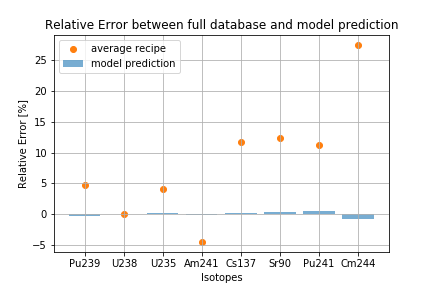
\includegraphics[width=\textwidth]{iso_rel.png}
    \caption{}
    \label{fig:iso_rel}
\end{figure}


\begin{figure}
    \centering
    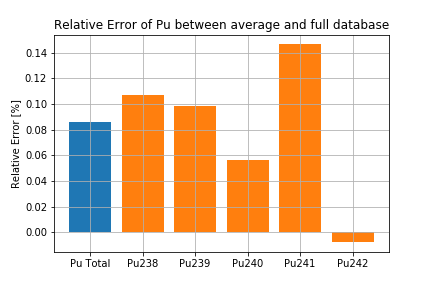
\includegraphics[width=\textwidth]{pu_rel.png}
    \caption{}
    \label{fig:pu_rel}
\end{figure}



\subsubsection{Waste Metric}
The model excellently predicts the waste metrics activity
and decay heat. Figures \ref{fig:assem_dh} and \ref{fig:assem_act}
show the relative error percent of the decay heat and activity
predictions per assembly. The model predicts most assemblies
with an error less than 1\%, except for assemblies with low burnup.


\begin{figure}
    \centering
    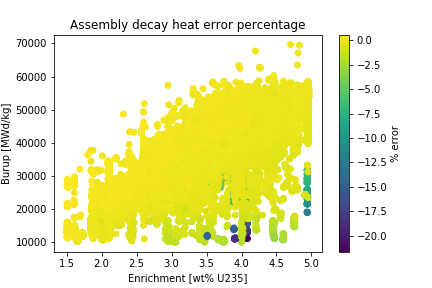
\includegraphics[width=\textwidth]{assem_dh.png}
    \caption{}
    \label{fig:assem_dh}
\end{figure}


\begin{figure}
    \centering
    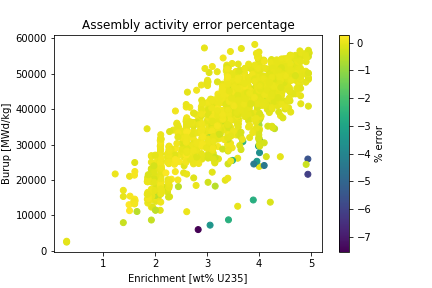
\includegraphics[width=\textwidth]{assem_act.png}
    \caption{}
    \label{fig:assem_act}
\end{figure}

Table \ref{tab:wm} shows the decay heat and activity value
comparison in years 2020, 2100, and 3100. The total
error is less than 1.1\% for all metrics at all time periods.
Figure \ref{fig:ha_err} shows the relative error percentage
of activity and decay heat progression in time. It shows
that the model outperforms the average recipe method
in predicting waste metrics.


\begin{table}[h]
    \centering
    \begin{tabular}{lcrrr}
        \hline
        Metric & Year & HR case & Prediction case  & Error [\%] \\
        \hline
        \multirow{3}{*}{\shortstack{Decay \\ Heat}} & 2020 & 41.01 & 40.83 & 0.43 \\
                                                    & 2100 & 16.43 & 16.39 & 0.23 \\
                                                    & 3100 & 3.14 & 3.13 & 0.085 \\
        \hline
        \multirow{3}{*}{\shortstack{Activity}} & 2020 & 4.67e20 & 4.62e20 & 1.07 \\
                                               & 2100 & 6.39e19 & 6.32e19 & 1.09 \\
                                               & 3100 & 3.68e18 & 3.68e18 & 0.061 \\
        \hline
    \end{tabular}
    \caption{Decay heat and radioactivity values and errors for years 2020, 2100, and 3100.}
    \label{tab:wm}
\end{table}

\begin{figure}
    \centering
    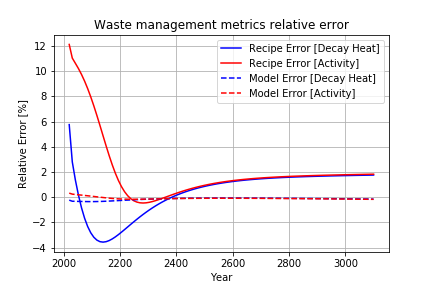
\includegraphics[width=\textwidth]{ha_err.png}
    \caption{Relative error of waste management metrics for \gls{UNF} inventory
             generated by the average recipe, and the prediction model.}
    \label{fig:ha_err}
\end{figure}


\subsubsection{Fissile quantity}

\begin{figure}
    \centering
    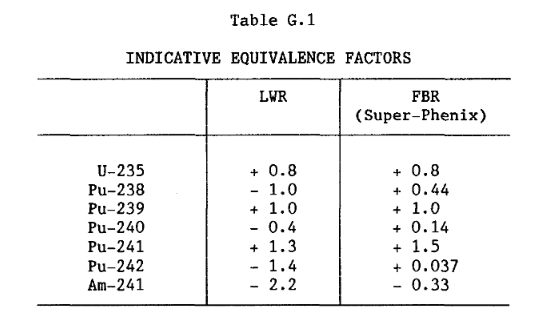
\includegraphics[width=\textwidth]{pu_equiv.png}
    \caption{}
    \label{fig:pu_equiv}
\end{figure}


\begin{figure}
    \centering
    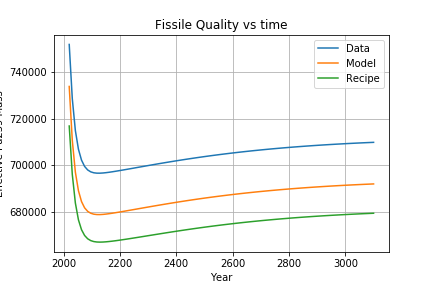
\includegraphics[width=\textwidth]{fiss.png}
    \caption{}
    \label{fig:fiss}
\end{figure}




\FloatBarrier